
% Auriga theme
% https://github.com/anishathalye/auriga

\documentclass[14pt,aspectratio=169]{beamer}
\usepackage{pgfpages}
\usepackage{fancyvrb}
\usepackage{booktabs,dcolumn}
\usepackage{tikz}
\usetikzlibrary{arrows.meta, positioning, quotes}
\usepackage{pgfplots}

% \ifnotes
% \setbeamertemplate{note page}[plain]
% \setbeameroption{show notes on second screen=right}
% \fi

\usetheme{auriga}
\usecolortheme{auriga}

% define some colors for a consistent theme across slides
\definecolor{red}{RGB}{181, 23, 0}
\definecolor{blue}{RGB}{0, 118, 186}
\definecolor{gray}{RGB}{146, 146, 146}

\title{Historia Económica Argentina}

\author{\underline{Sebastián Freille} \inst{1}}

\institute[shortinst]{\inst{1} IEF-UNC \\ UCC}
\date{}

\AtBeginSection[]{
    \begin{frame}
    \vfill
    \centering
    \begin{beamercolorbox}[sep=8pt,center,shadow=true,rounded=true]{title}
        \usebeamerfont{title}\insertsectionhead\par%
    \end{beamercolorbox}
    \vfill
    \end{frame}
}



\AtBeginSubsection[]{
    \begin{frame}
    \vfill
    \centering
    \begin{beamercolorbox}[sep=6pt,center,shadow=true,rounded=true]{title}
        \usebeamerfont{title}\insertsubsectionhead\par%
    \end{beamercolorbox}
    \vfill
    \end{frame}
}


\AtBeginSubsubsection[]{
    \begin{frame}
    \vfill
    \centering
    \begin{beamercolorbox}[sep=4pt,center,shadow=true,rounded=true]{title}
        \usebeamerfont{title}\insertsubsubsectionhead\par%
    \end{beamercolorbox}
    \vfill
    \end{frame}
}


\begin{document}

{
  % rather than use the frame options [noframenumbering,plain], we make the
  % color match, so that the indicated page numbers match PDF page numbers
  \setbeamercolor{page number in head/foot}{fg=background canvas.bg}
  \begin{frame}
    \titlepage
  \end{frame}
}


\section{Capítulo 6. Estancamiento y declinación, 1973-89}

\begin{frame}\frametitle{El regreso de Perón}
                 \begin{itemize}\itemsep 5pt \medskip
                 \item Primera votación presidencial en una década en
                   1973 $\longrightarrow$ ``Cámpora al gobierno, Perón
                   al poder'' (FREJULI)
                   \item ¿Qué era el peronismo en ese momento? Gran
                     problema de identidad
                     \item Promueve un ``Pacto Social'' entre
                       empresarios, trabajadores y gobierno
                       \item Ideas similares, formas diferentes
                   \end{itemize}
               \end{frame}



\begin{frame}\frametitle{El regreso de Perón (cont.)}
                 \begin{itemize}\itemsep 5pt \medskip
                 \item Campora renuncia a los 50 días y
                   asume Perón-Estela de Perón con 62\% de los votos
                   \item Con oposición del ala más radical (izquierda)
                     del peronismo y dudas en el eje
                     sindical/político, Perón no tuvo apoyos
                     \item Luego de su muerte en 1974, asume Isabelita
                       $\longrightarrow$ gobierno aún más débil que el
                       anterior
                       \item Había un gran vacío de poder (real, no
                         formal) y eso derivó en un nuevo golpe militar
                   \end{itemize}
               \end{frame}


\begin{frame}\frametitle{El regreso de Perón (cont.)}
                 \begin{itemize}\itemsep 5pt \medskip
                 \item El ministro de economía Gelbard generaba
                   tensiones por ser empresario $\longrightarrow$
                   entraba en lógica peronista de negociación
                   (empresarios y sindicatos)
                   \item Pacto social entre Confederación General
                     Económica (CGE), CGT y Ministerio de Economía
                     $\longrightarrow$ 1) reformas de fondo; 2) plan
                     concertado de estabilización
                   \end{itemize}
               \end{frame}
               



\begin{frame}\frametitle{El regreso de Perón (cont.)}
                 \begin{itemize}\itemsep 5pt \medskip
                 \item El programa (plan Gelbard) era reformista pero
                   no revolucionario
                   \item Ley de inversiones extranjeras (1973)
                     limitaba peso del capital externo
                     \item Énfasis en exportaciones industriales
                       --industria no orientada al mercado interno
                       sino al externo
                       \item La ``Ley de Protección al Trabajo y la
                         Producción Nacional'' contribuyó a ese
                         impulso con incentivos para exportar y
                         crédito a PyMEs
                   \end{itemize}
               \end{frame}
               


 \begin{frame}\frametitle{El regreso de Perón (cont.)}
\begin{figure}[hxtbp]\vspace{0cm}
  \centering
  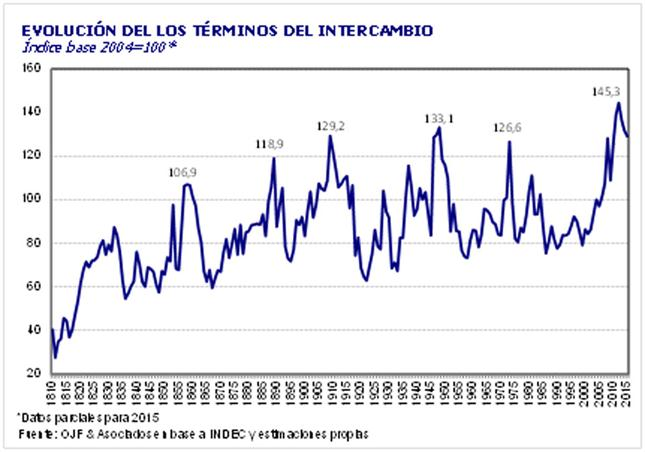
\includegraphics[scale=0.5]{uni6_peron02}
   \caption{TIE de dos siglos}
\end{figure} 
  \end{frame}
               


\begin{frame}\frametitle{El regreso de Perón (cont.)}
                 \begin{itemize}\itemsep 5pt \medskip
                 \item Cuentas externas en el mejor momento del siglo
                   de la mano de TIE históricos (``boom de las
                   materias primas'')
\item Nueva nacionalización del comercio exterior (Junta Nacional de
  Granos y Junta Nacional de Carnes)
  \item Proyecto de Ley Agraria $\longrightarrow$ expropiación de
    tierras consideradas ``improductivas'' --muy mal recibida por
    terratenientes
    \item Se creó el impuesto a la renta potencial de la tierra
      --incentivo a producir/usar más la tierra
                 \end{itemize}
               \end{frame}



 \begin{frame}\frametitle{El regreso de Perón (cont.)}
\begin{figure}[hxtbp]\vspace{0cm}
  \centering
  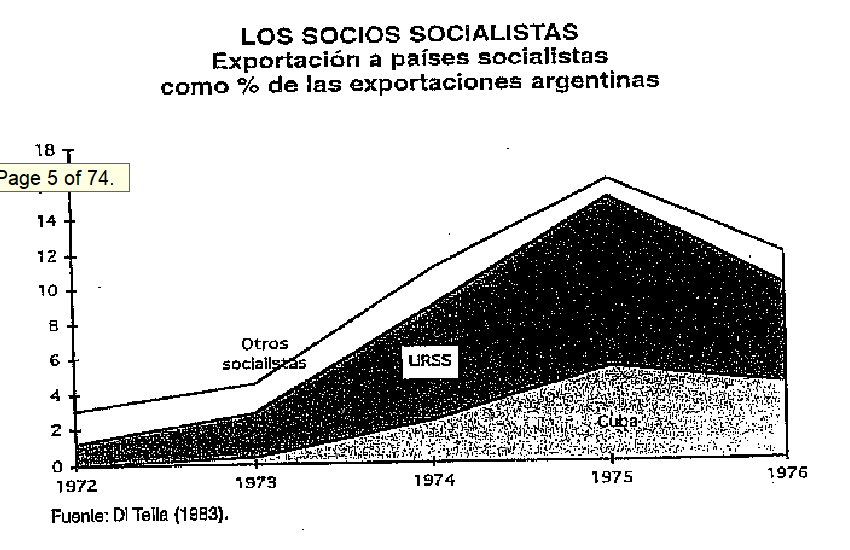
\includegraphics[scale=0.6]{uni6_peron03}
   \caption{Los nuevos socios en el comercio}
\end{figure} 
  \end{frame}
               

\begin{frame}\frametitle{El regreso de Perón (cont.)}
                 \begin{itemize}\itemsep 5pt \medskip
                 \item Nuevos socios comerciales (Europa del Este,
                   Medio Oriente), paises socialitas $\longrightarrow$
                   pasaron de 3 al 11\% como destino de X
                   \item No hubo nacionalización de depósitos pero si
                     una centralización del sistema bancario
                     $\longrightarrow$ BCRA coordinaba depósitos y
                     créditos lo que permitía controla M más
                     centralmente
                     \item En el único aspecto en que hubo un
                       contraste bien marcado con su primer epoca fue
                       $\longrightarrow$ combate a la inflación
                 \end{itemize}
               \end{frame}


  
\begin{frame}\frametitle{El regreso de Perón (cont.)}
                 \begin{itemize}\itemsep 5pt \medskip
                 \item Gelbard partió de un diagnóstico de la
                   inflación como fenómeno estructural (y no como
                   producto de PF y PM expansiva)
                   \item Campora/Perón reconocían que la distribución
                     del PBI era inadecuada para combatir la inflación
                     $\longrightarrow$ 2/3 para el K y 1/3 para el
                     trabajo
                     \item Se realizó una ingeniería de precios
                       nominales (algunos incluso bajaron) y
                       relativos; suspensión de CCT por 2 años
                 \end{itemize}
               \end{frame}


               \begin{frame}\frametitle{El regreso de Perón (cont.)}
                 \begin{itemize}\itemsep 5pt \medskip
                 \item Sindicalismo descontento con esta política
                   concertada de precios y salarios (Pacto Social) $\longrightarrow$
                   quitaba poder de negociación
                   \item Empresarios tampoco de acuerdo pero lo
                     preferían a un mal mayor (expropiación, nacionalización)
                     $\longrightarrow$ anhelaban por una solución al
                     problema inflacionario
                     \item Los números de la economía fueron buenos
                       (mejores que en 1972) en 1973
                 \end{itemize}
               \end{frame}



                \begin{frame}\frametitle{El regreso de Perón (cont.)}
                 \begin{itemize}\itemsep 5pt \medskip
                 \item Inflación en 1973 fue de 60\% $\longrightarrow$
                   toda en el primer semestre, inflación cero en el
                   segundo semestre!
                   \item Experiencia de Gelbard interesante
                     $\longrightarrow$ rol de las expectativas sobre
                     precios futuros [dinámica inflación-estabilización]
                     \item Incluso Gelbard siguió aumentando cantidad
                       de dinero sin que aumentaran precios en lo
                       inmediato...
                       \item ...pero no es sostenible en mediano plazo
                 \end{itemize}
               \end{frame}

               

\begin{frame}\frametitle{El regreso de Perón (cont.)}
                 \begin{itemize}\itemsep 5pt \medskip
                 \item Nuevamente el golpe vino de afuera
                   $\longrightarrow$ aumento de precios de M (insumos)
                   y empresarios pidieron por flexibilidad para fijar
                   precios --gobierno subsidia compra de insumos
                   \item Pero en 1974, multiples reclamos para revisar
                     salarios y precios (por aumentos en el costo de
                     vida, aumento precio del petroleo, aumento de
                     tarifas) $\longrightarrow$ gran paritaria
                     nacional de 1974 (aumentos de sueldos, tarifas y
                     combustibles)
                     \item El Pacto Social estaba herido de muerte
                       $\longrightarrow$ recalentamiento de la economía
                 \end{itemize}
               \end{frame}


               \begin{frame}\frametitle{El regreso de Perón (cont.)}
                 \begin{itemize}\itemsep 5pt \medskip
                 \item El PBI y empleo siguieron creciendo en 1974
                   pero resurgió la inflación y empeoró la cuenta
                   externa
                    \item La muerte de Perón tiró por la borda
                      cualquier posibilidad de parar la espiral
                      --reversión de expectativas, estanflación
                      internacional, atraso cambiario (TCFi)
                      \item Era tiempo de desandar el camino del Pacto
                        Social pero en un marco de un gobierno débil y
                        con alta conflictividad social
                 \end{itemize}
               \end{frame}
               

  
\section{El (breve) gobierno de Isabelita}



\begin{frame}\frametitle{Una transición inestable}
                 \begin{itemize}\itemsep 5pt \medskip
                 \item Mientras Gelbard fue el único ministro de Economía de cuatro
                   presidentes, hubo 6 (seis) ministros en el breve
                   gobierno de Isabelita
                   \item Fue un gobierno que sólo pudo mostrar un
                     expansión económica (inercial) porque el resto de
                     indicadores fueron muy pobres
                     \item Al principio, hubo correcciones graduales
                       de precios y salarios pero poco avance en
                       frente fiscal y externo
                 \end{itemize}
               \end{frame}
               

               
               \begin{frame}\frametitle{Una transición inestable (cont.)}
                 \begin{itemize}\itemsep 5pt \medskip
                 \item Rodrigo anunció las siguientes medidas
                   (\textit{El Rodrigazo}):
                   \begin{itemize}\itemsep 5pt \medskip
                   \item Devaluación de 100\%
                     \item Aumento de tarifas públicas con 100\% de
                       piso
                       \item Liberalización de (casi) todos los
                         precios
                       \end{itemize}
                       \item Fuertes movilizaciones gremiales forzaron
                         renuncias de Lopez Rega (superministro) y
                         Rodrigo
                         \item Mientras la economía pasaba de
                           expansión a recesión (1975)
                 \end{itemize}
               \end{frame}


               \begin{frame}\frametitle{Una transición inestable (cont.)}
                 \begin{itemize}\itemsep 5pt \medskip
                 \item A mediados de 1975 la situación económica y
                   política era muy delicada:
                   \begin{itemize}\itemsep 5pt \medskip
                   \item Se acuerda un préstamo del FMI y mantener un
                     alto precio del dólar
                     \item Política económica no tenía credibilidad
                       --imposible generar confianza
                       \item Déficit fiscal descontralado --llegó a
                         ser de 12.4\% del PBI!
                         \item Precios mayoristas aumentaron más del
                           50\% en un solo mes (marzo 1975)
                         \end{itemize}
                         \item Nuevamente se produce un golpe
                           cívico-militar en marzo de 1976
                 \end{itemize}
               \end{frame}


               

               
\section{El gobierno militar: El Proceso}



     \begin{frame}\frametitle{El gobierno militar: 1976-83}
                 \begin{itemize}\itemsep 5pt \medskip
                 \item Objetivo prioritario del Proceso de
                   Reorganización Nacional (PRN) era acabar con grupos
                   armadas (ERP, Montoneros). Esto se completó en
                   1978.  
                   \item Compartían algunas
                   premisas con la Revolución Argentina pero tenía ideología $\longrightarrow$ sociedad
                     despolitizada y Estado menos poderoso
                     \item Violación sistemática de DDHH afectaba
                       imagen internacional del país $\longrightarrow$
                       tensión con Chile
                 \end{itemize}
               \end{frame}


                \begin{frame}\frametitle{El gobierno militar: 1976-83 (cont.)}
                 \begin{itemize}\itemsep 5pt \medskip
                 \item Presidentes de facto de Argentina en 1976-83:
                   \begin{itemize}\itemsep 5pt\medskip
                   \item Jorge Rafael Videla (1976-81)
                   \item Roberto Viola (1981-81)
                   \item Leopoldo Galtieri (1981-82)
                     \item Reynaldo Bignone (1982-83)
                     \end{itemize}
                     \item Todos estos presidentes de facto
                       organizaron el poder alrededor de la denominada
                       Junta Militar de Gobierno 
                 \end{itemize}
               \end{frame}



                \begin{frame}\frametitle{El gobierno militar: 1976-83 (cont.)}
                 \begin{itemize}\itemsep 5pt \medskip
                 \item Hacia inicios de la década de 1980, el gobierno
                   militar había perdido casi toda razón de ser
                   $\longrightarrow$ no había enemigos militares que
                   combatir ni tampoco resultados económicos
                   significativos
                   \item También hacia esa época se forma
                     \textit{La Multipardiaria Nacional} --canal de
                     agrupaciones para pujar por salida institucional
                     \item Si bien un proceso similar al de la
                       Revolución Argentina, Galtieri no iba a
                       conceder facilmente la via democratica
                 \end{itemize}
               \end{frame}



                \begin{frame}\frametitle{El gobierno militar: 1976-83 (cont.)}
                 \begin{itemize}\itemsep 5pt \medskip
                 \item Ministro clave del Proceso: Martínez de Hoz
                   (empresario liberal vinculado a la democracia
                   cristiana).
                   \item Opinaba que la inflación obedecía a falencias
                     profundas en la organización económica
                     \item Proponía reinvidicar la iniciativa privada
                       y eliminar el déficit fiscal
                       \item Estos eran no sólo objetivos sino además
                         precondiciones para la tan ansiada
                         estabilidad de precios
                 \end{itemize}
               \end{frame}


  \begin{frame}\frametitle{El gobierno militar: 1976-83 (cont.)}
                 \begin{itemize}\itemsep 5pt \medskip
                 \item La visión y discurso de Martínez de Hoz no era
                   ajena al contexto $\longrightarrow$ el
                   keynesianismo y el Estado de bienestar de los
                   50s-60s estaban en decadencia
                   \item Esto se debió a cambios en la teoría
                     --Friedman y Phelps cuestionaron la curva de
                     Phillips (vertical a LP)- y en los
                     hechos --inflación mundial en aumento a fines de
                     los 60
                     \item Esto dio origen a una visión que no se
                       podía bajar el desempleo más allá de su tasa
                       natural sin acelerar fuertemente la inflación
                 \end{itemize}
               \end{frame}


  \begin{frame}\frametitle{El gobierno militar: 1976-83 (cont.)}
                 \begin{itemize}\itemsep 5pt \medskip
                 \item La economía mundial además pasa por eventos
                   antes impensados --abandono de Bretton-Woods y
                   estanflación de 1973-75. Revolución de las
                   expectativas racionales --ni siquiera era efectivo
                   el uso de la política activa en el CP!
                   \item Adicionalmente, la teoría del enfoque
                     monetario de la BP
                   \item Tanto en la teoría como en la práctica se
                     cuestionaba la capacidad misma del Estado para
                     hacer política económica
                 \end{itemize}
               \end{frame}
               


 \begin{frame}\frametitle{El gobierno militar: 1976-83 (cont.)}
   \begin{block}{EMBP}
Con TCFijo, todo aumento de la OM (sin aumento de DM) se
contrarrestaba con una pérdida de reservas ya que el exceso de dinero
no deseado buscaba destino. Con TCFlexible, todo aumento de la OM (sin
aumento de DM) se contrarrestaba con un aumento del tipo de cambio
(depreciación). La prescripción clara que resultada de la revolución
de la macro y las ER era: expandir OM sólo para atender necesidades de
liquidez (transacciones)
     \end{block}
               \end{frame}



 \begin{frame}\frametitle{El gobierno militar: 1976-83 (cont.)}
                 \begin{itemize}\itemsep 5pt \medskip
                 \item Hubo un desfasaje temporal entre ideas teóricas
                   (1970s) y su aplicación (1980s): Thatcher en UK y
                   Reagan en US desmantelaron los Estados de bienestar
                   y aplicaron PM ortodoxa
                   \item Chile -también bajo un proceso militar-
                     adoptó políticas económicas de liberalización
                     radicales --privatización de bancos,
                     flexilibización de precios, baja de déficit
                     fiscal y apertura externa [fuerte aumento del desempleo]
                     \item Baja inflación, crawling peg y alto
                       crecimiento en el caso Chileno 
                 \end{itemize}
               \end{frame}


                \begin{frame}\frametitle{El gobierno militar: 1976-83 (cont.)}
                 \begin{itemize}\itemsep 5pt \medskip
                 \item Martínez de Hoz planteó una lista de
                   prioridades: 1) estabilidad de precios, 2)
                   crecimiento económico, 3) distribución de ingresos
                   ``razonable''.
                   \item Recordemos que Argentina en 1976 tenía una
                     economía con un principio de hiperinflación y una
                     situación de pagos externa crítica
                     \item Todos estas prioridades y objetivos
                       fracasaron en su cumplimiento y de hecho, lejos
                       estuvieron de alcanzarse
                 \end{itemize}
               \end{frame}



 \begin{frame}\frametitle{El gobierno militar: 1976-83 (cont.)}
                 \begin{itemize}\itemsep 5pt \medskip
                 \item La estrategia anti-inflacionaria fue
                   \textit{gradualista} $\longrightarrow$ se
                   congelaron salarios, se liberaron
                   precios (no se devaluó) y se fue ajustando el tipo
                   de cambio según la inflación
                   \item Cayó el salario real lo que mejoraría las
                     cuentas externas (competitividad)
                     \item Adicionalmente se obtuvo una nueva ayuda
                       del FMI para compromisos de corto plazo
                 \end{itemize}
               \end{frame}




               
 \begin{frame}\frametitle{El gobierno militar: 1976-83 (cont.)}
                 \begin{itemize}\itemsep 5pt \medskip
                 \item En 1977 la economía tenía un poco más de orden
                   y credibilidad --combinación de políticas
                   cambiarias, salarial y arancelaria lograron generar
                   excedentes comerciales
                   \item Déficit fiscal estaba bajando y también lo
                     hacía la inflación
                     \item Pero desde 1977 la inflación vuelve a tomar
                       vuelo (7\% mensual) --algunos controles y
                       ``treguas'' de precios
                 \end{itemize}
               \end{frame}


\begin{frame}\frametitle{El gobierno militar: 1976-83 (cont.)}
                 \begin{itemize}\itemsep 5pt \medskip
                 \item Un cambio muy drástico fue la \textbf{reforma
                     financiera} $\longrightarrow$ papel de los bancos
                   en la distribución del credito
                   \item Un gran problema histórico fueron las tasas
                     reales negativas de interés (combinación de tasas
                     reguladas e inflación creciente)
                     \item Esto fue un fenómeno muy persistente
                       durante gran parte de la posguerra
                       \end{itemize}
               \end{frame}


 \begin{frame}\frametitle{El gobierno militar: 1976-83 (cont.)}
\begin{figure}[hxtbp]\vspace{0cm}
  \centering
  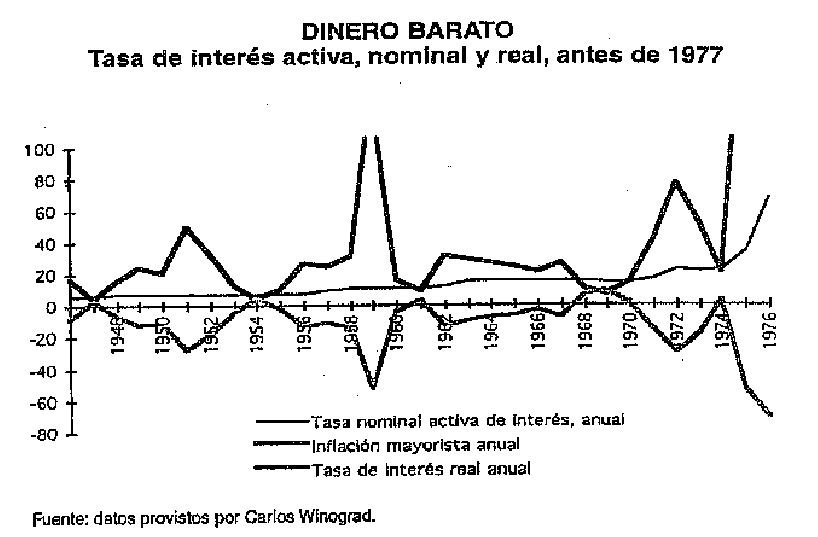
\includegraphics[scale=0.6]{uni6_peron05}
   \caption{Dinero barato}
\end{figure} 
  \end{frame}


\begin{frame}\frametitle{El gobierno militar: 1976-83 (cont.)}
                 \begin{itemize}\itemsep 5pt \medskip
                 \item Esta reforma financiera pretendía ser un cambio
                   sustancial en el mercado de K
                   argentino. Principales medidas fueron:
                   \begin{itemize}\itemsep 5pt \medskip
                   \item liberación de tasas de interés
                     \item descentralización de depósitos --ie
                       capacidad de bancos de prestar atada a
                       depositos captados
                       \item encajes regulados de manera de controlar
                         tasas de interes
                   \end{itemize}
                 \item Una idea central era acabar con la especulación
                   y el circuito informal $\longrightarrow$ no era
                   rentable prestar en esas condiciones (para bancos)
                   \end{itemize}
               \end{frame}




\begin{frame}\frametitle{El gobierno militar: 1976-83 (cont.)}
                 \begin{itemize}\itemsep 5pt \medskip
                 \item Algunos efectos de esta reforma fueron en la
                   dirección correcta:
                   \begin{itemize}\itemsep 5pt \medskip
                     \item Aumento número de bancos de 119 a 219 entre
                       1977 y 1980
                       \item Aumento depositos a plazo de 5.9\% a
                         16.5\% del PBI (efecto de tasas reales
                         positivas)
                         \item El ahorro doméstico (en oposición al
                           consumo) no aumentó tanto --mercado de
                           crédito fomentó consumo no tanto inversión
                         \end{itemize}
                       \item Uno de los grandes problemas fue la
                         expansión financiera sin un control adecuado
                         (escenario de alto riesgo)
                         \end{itemize}
               \end{frame}



               \begin{frame}\frametitle{El gobierno militar: 1976-83 (cont.)}
                 \begin{itemize}\itemsep 5pt \medskip
                 \item Competencia bancaria hizo que ofrecieran tasas
                   altas por pasivos y replicarlas en los activos
                   --empresas tomaban préstamos a altas tasas
                   \item Era diferente la apuesta de acreedores y
                     deudores --deudores esperaban licuación de
                     pasivos ante una escalada inflacionaria;
                     acreedores esperaban rescate del BCRA
                     \item El sistema aguantó mientras el dinero
                       estuviera en los bancos --una corrida en 1980
                       hizo que el BCRA asumiera el control de 60 instituciones
                   \end{itemize} 
               \end{frame}
               




               \begin{frame}\frametitle{El gobierno militar: 1976-83 (cont.)}
                 \begin{itemize}\itemsep 5pt \medskip
                 \item La crisis bancaria y financiera fue el inicio
                   del fin del programa de Martínez de Hoz --la
                   economía nunca había dejado de ser una economía de
                   especulación
                   \item En cuatro años de gobierno (1976-80) apenas
                     se había crecido. La principal prioridad
                     (inflación) seguía siendo aún un problema sin
                     solución
                     \item El gradualismo de Martínez de Hoz fue
                       ecléctico y carente de una estrategia clara y homogénea
                   \end{itemize} 
               \end{frame}
               

\begin{frame}\frametitle{El gobierno militar: 1976-83 (cont.)}
                 \begin{itemize}\itemsep 5pt \medskip
                 \item Primero, se buscaron salidas heterodoxas
                   --tregua de precios, reducciones arancelarias
                   \item Segundo, se pasó a una receta ortodoxa
                     --disminuir OM- sin financiar a Estado y empresas
                     públicas. Pero la inflación crecía a 10\%
                     mensual. El aumento de tasas generó una fuerte
                     contracción económica --hasta ahí era predecible
                     hasta que se ajustaran expectativas de
                     inflación. El problema existía en otro ambito
                     $\longrightarrow$ intervención en mercado de
                     cambios (``crawling peg'')
                     \item Nuevamente aparecen las inconsistencias
                       $\longrightarrow$ podía elegir precio del dólar
                       o la cantidad de dinero pero no ambas
                   \end{itemize} 
               \end{frame}
               


\begin{frame}\frametitle{El gobierno militar: 1976-83 (cont.)}
                 \begin{itemize}\itemsep 5pt \medskip
                 \item Monetarismo duro y ``crawling peg'' no eran
                   compatibles --en 1978 parecía que el gobierno
                   renunciaba a la política cambiaria. Dejó de
                   intervenir y esto provocó una fuerte apreciación
                   real (TCN en equilibrio pero precios con fuerte aumento)
                   \item Dado que el control monetario no daba
                     resultados, se hizo otro viraje ahora con
                     objetivo de controlar el tipo de cambio --aparece
                     la famosa \textbf{tablita}. La tablita era un
                     cronograma que especificaba el valor del dólar
                     durante 8 meses a partir de 1979
                   \end{itemize} 
               \end{frame}
               

\begin{frame}\frametitle{El gobierno militar: 1976-83 (cont.)}
                 \begin{itemize}\itemsep 5pt \medskip
                 \item Monetarismo duro y ``crawling peg'' no eran
                   compatibles --en 1978 parecía que el gobierno
                   renunciaba a la política cambiaria. Dejó de
                   intervenir y esto provocó una fuerte apreciación
                   real (TCN en equilibrio pero precios con fuerte aumento)
                   \item Dado que el control monetario no daba
                     resultados, se hizo otro viraje ahora con
                     objetivo de controlar el tipo de cambio --aparece
                     la famosa \textbf{tablita}. La tablita era un
                     cronograma que especificaba el valor del dólar
                     durante 8 meses a partir de 1979
                   \end{itemize} 
               \end{frame}
               

         \begin{frame}\frametitle{El gobierno militar: 1976-83 (cont.)}
\begin{figure}[hxtbp]\vspace{0cm}
  \centering
  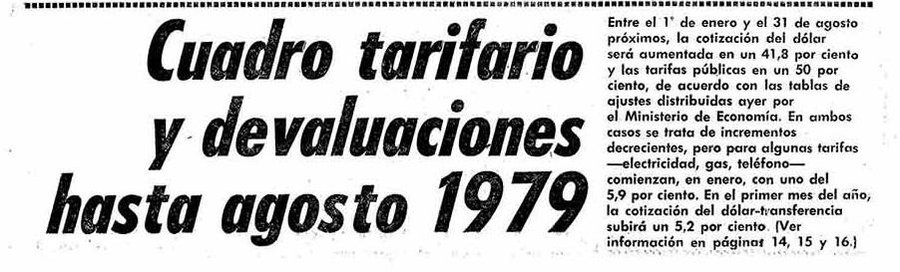
\includegraphics[scale=0.4]{uni6_tablita}
   \caption{Anuncio de la tablita}
\end{figure} 
  \end{frame}       
               


  \begin{frame}\frametitle{El gobierno militar: 1976-83 (cont.)}
                 \begin{itemize}\itemsep 5pt \medskip
                 \item La apuesta era bajar la inflación atando la
                   moneda local al precio del dólar $\longrightarrow$
                   si el precio (en dólares) de los transables subía
                   10\% y la tablita preveia un aumento del 60\% en el
                   tipo de cambio, el precio local de los transables
                   debía aumentar cerca del 70\%
                   \item Tenía algunos atractivos: 1) hacia previsible
                     el ritmo devaluatorio; 2) daba sendero bajista de
                     la inflación; 3) no afectaba tasa de interés al alza (no
                     era recesivo) sino a la baja al bajar el riesgo
                     de operación
                   \end{itemize} 
               \end{frame}
               


  \begin{frame}\frametitle{El gobierno militar: 1976-83 (cont.)}
                 \begin{itemize}\itemsep 5pt \medskip
                 \item En 1979, las tasas reales bajaron y la
                   actividad se expandió --pero tasas reales bajaron
                   no por baja de riesgo sino por persistencia de
                   inflación
                   \item El plan falló en su objetivo más importante:
                     bajar la inflación. Y como el aumento del precio
                     del dólar esta fijado de antemano y la inflación
                     lo triplicaba (entre 150 y 175\% anual), el
                     atraso cambiario cada vez se hizo peor
                     \item ¿Por qué falló la tablita en hacer
                       converger la inflación a la tasa de cambio del dólar?
                   \end{itemize} 
               \end{frame}
               
               




         \begin{frame}\frametitle{El gobierno militar: 1976-83 (cont.)}
\begin{figure}[hxtbp]\vspace{0cm}
  \centering
  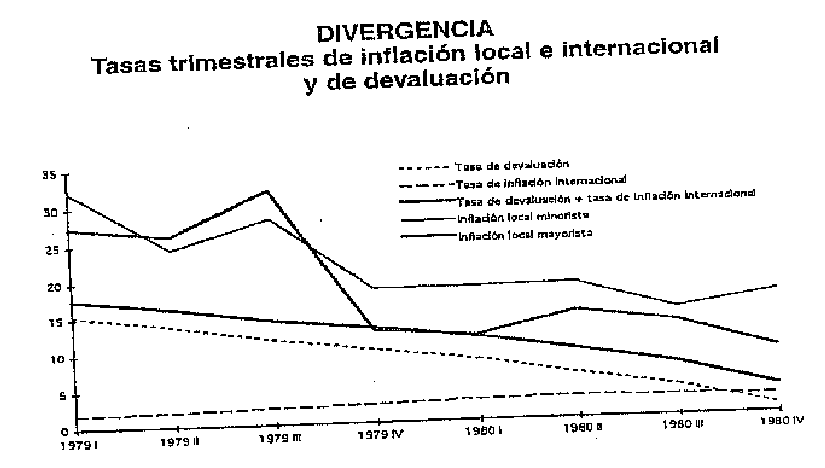
\includegraphics[scale=0.6]{uni6_tablita02}
   \caption{Desempeño de la tablita}
\end{figure} 
  \end{frame}  





 \begin{frame}\frametitle{El gobierno militar: 1976-83 (cont.)}
                 \begin{itemize}\itemsep 5pt \medskip
                 \item Luego de una reversión de la balanza comercial,
                   una fuerte crisis interna en 1980 y una disparada
                   de las tasas de interés, se anuncian medidas para
                   reducir el déficit fiscal y para flexibilizar la
                   toma de deuda externa
                   \item En 1980 se produce una corrida contra el peso
                     (más de la mitad de las reservas)
                     y una devaluación no programada de 10\% acabó ocn
                     la tablita.
                     \item Al momento de cambio de gobierno, la
                       economía estaba en recesión y con una inflación
                       que daba señales de acelerarse
                   \end{itemize} 
               \end{frame}
               




 \begin{frame}\frametitle{El gobierno militar: 1976-83 (cont.)}
                 \begin{itemize}\itemsep 5pt \medskip
                 \item Habiendo fracasado en el ojbetivo de controlar
                   la inflación, tampoco fue muy buena la performance
                   en comercio exterior
                   \item Se eliminaron retenciones y otros impuestos y
                     se aumentó la producción de bienes exportables
                     \item Política gradual de apertura a M para
                       evitar reestructuración productiva brusca (como
                       en la década de los 90)
                   \end{itemize} 
               \end{frame}
               

               
\begin{frame}\frametitle{El gobierno militar: 1976-83 (cont.)}
                 \begin{itemize}\itemsep 5pt \medskip
                 \item Si la estrategia comercial fue diseñada para
                   apertura gradual y con eliminación de aranceles e
                   impuestos ¿por qué se dio una fenomenal avalancha
                   de M?
                   \item Respuesta obvia $\longrightarrow$ atraso
                     cambiario determinante
                     \item Reducción de impuestos favoreció a
                       exportables pero la apreciación del peso
                       mejoraba la relación $P_{NT}$ versus $P_{T}$
                       \item Sector industrial local fuertemente
                         perjudicado $\longrightarrow$ aluvión de M
                         competía con sus productos
                   \end{itemize} 
               \end{frame}




  \begin{frame}\frametitle{El gobierno militar: 1976-83 (cont.)}
\begin{figure}[hxtbp]\vspace{0cm}
  \centering
  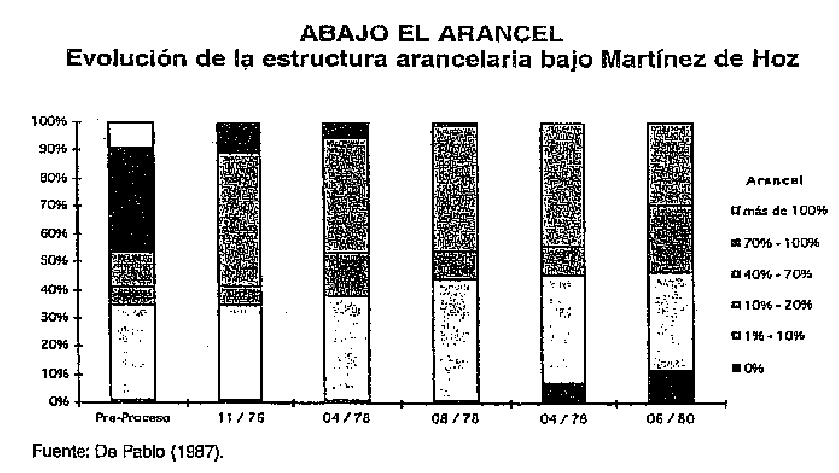
\includegraphics[scale=0.6]{uni6_tablita03}
   \caption{Política comercial}
\end{figure} 
  \end{frame}       
               

\begin{frame}\frametitle{El gobierno militar: 1976-83 (cont.)}
                 \begin{itemize}\itemsep 5pt \medskip
                 \item Está claro que la estrategia comercial del
                   gobierno militar le dió al sector externo por un
                   lado y le quitó (¿mucho más?) por el otro
                   $\longrightarrow$ protección efectiva era menor en
                   casi todas las industrias [queja principal el Plan
                   de Estabilización]
                   \item Industria redujo su participación en PBI
                     entre 3-4 puntos en 1974-80; agropecuario se
                     mantuvo; crecierlos los no transables
                     (construcción, otros servicios)
                     \item El gobierno de Videla culmina abandondando
                       sus principales banderas económicas: 1)
                       tablita; 2) sistema bancario; 3) apertura
                       insostenible
                   \end{itemize} 
               \end{frame}



  

  \begin{frame}\frametitle{El gobierno militar: 1976-83 (cont.)}
\begin{figure}[hxtbp]\vspace{0cm}
  \centering
  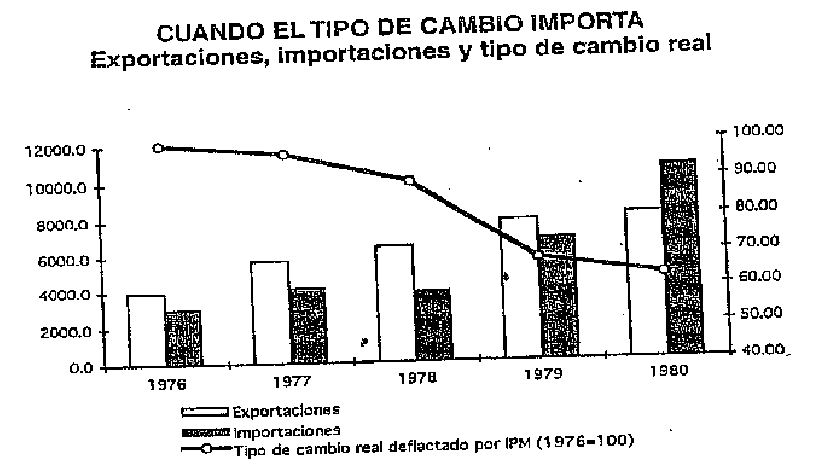
\includegraphics[scale=0.6]{uni6_tablita04}
   \caption{El problema del atraso cambiario}
\end{figure} 
  \end{frame}  




\begin{frame}\frametitle{El gobierno militar: 1976-83 (cont.)}
                 \begin{itemize}\itemsep 5pt \medskip
                 \item A principios de 1981, Argentina era una
                   combinación de: alta inflación, alto endeudamiento, y
                   con recesión. No sorprende que el período 1981-83
                   fuera cuantitativamente similar al de Isabelita
                   \item En resumidas cuentas, este período --con un
                     gobierno ya debilitado y fracturado- se vieron
                     sucesivas devaluaciones, desdoblamientos
                     cambiarios y escaladas inflacionarias.
                                        \end{itemize} 
               \end{frame}


\begin{frame}\frametitle{El gobierno militar: 1976-83 (cont.)}
                 \begin{itemize}\itemsep 5pt \medskip
                 \item Las primeras medidas fueron incluso contrarias a las de
                   Martínez de Hoz: se eliminó la tablita, se
                   re-regularon las tasas de interés y se volvió atrás
                   con la apertura comercial
                   \item Con Galtieri se inició una nueva
                     contra-contrarreforma que implicaba, al menos en
                     sus objetivos, tres cosas: desinflación, desregulación y desestatización
                   \end{itemize} 
               \end{frame}



               \begin{frame}\frametitle{El gobierno militar: 1976-83 (cont.)}
                 \begin{itemize}\itemsep 5pt \medskip
                 \item Uno de los problemas más relevantes de este
                   período fue el problema de la crisis de deuda
                   latinoamericana
                   \item En 1982 Méjico anuncia posible no pago de su
                     deuda y se cortó posibilidad de tomar nuevos
                     préstamos
                     \item El crecimiento de la deuda en este período
                       alcanzó dimensiones nunca antes vistas: estaba
                       endeudado el sector privado, el sector público,
                       los bancos
                   \end{itemize} 
               \end{frame}

                  
  \begin{frame}\frametitle{El gobierno militar: 1976-83 (cont.)}
                 \begin{itemize}\itemsep 5pt \medskip
                 \item El gobierno fue tal vez el principal
                   responsable de esto $\longrightarrow$ al priorizar
                   el objetivo inflacionario, se optó por tomar deuda
                   antes que emitir
                   \item El problema es que esto es una bomba de
                     tiempo si el déficit fiscal no se mantiene bajo
                     (o nulo)
                     \item Argentina pasó de un déficit de 3.7\% en
                       1977, a 5.5\% en 1980 y a niveles de Isabelita
                       en 1982/83
                   \end{itemize} 
               \end{frame}


  \begin{frame}\frametitle{El gobierno militar: 1976-83 (cont.)}
\begin{figure}[hxtbp]\vspace{0cm}
  \centering
  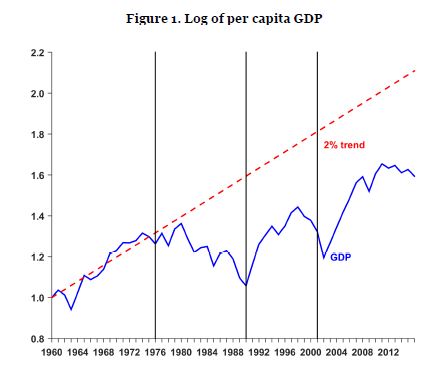
\includegraphics[scale=0.8]{uni6_deuda01}
   \caption{PBI per capita. Fuente: Buera and Nicolini (2019)}
\end{figure} 
  \end{frame}  
               

  \begin{frame}\frametitle{El gobierno militar: 1976-83 (cont.)}
\begin{figure}[hxtbp]\vspace{0cm}
  \centering
  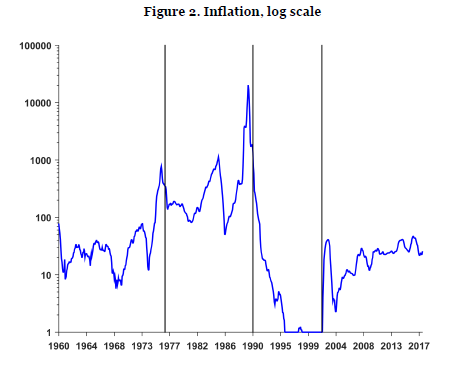
\includegraphics[scale=0.8]{uni6_deuda02}
   \caption{Inflación. Fuente: Buera and Nicolini (2019)}
\end{figure} 
  \end{frame}  



  \begin{frame}\frametitle{El gobierno militar: 1976-83 (cont.)}
\begin{figure}[hxtbp]\vspace{0cm}
  \centering
  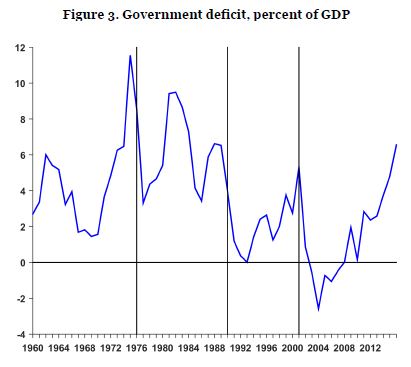
\includegraphics[scale=0.8]{uni6_deuda03}
   \caption{Déficit fiscal. Fuente: Buera and Nicolini (2019)}
\end{figure} 
  \end{frame}  


    \begin{frame}\frametitle{El gobierno militar: 1976-83 (cont.)}
\begin{figure}[hxtbp]\vspace{0cm}
  \centering
  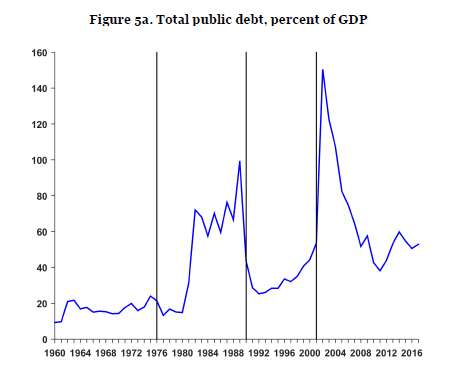
\includegraphics[scale=0.8]{uni6_deuda04}
   \caption{Deuda (porcantaje PBI). Fuente: Buera and Nicolini (2019)}
\end{figure} 
  \end{frame}  



    \begin{frame}\frametitle{El gobierno militar: 1976-83 (cont.)}
\begin{figure}[hxtbp]\vspace{0cm}
  \centering
  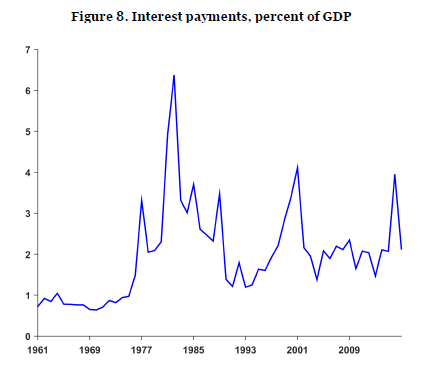
\includegraphics[scale=0.8]{uni6_deuda05}
   \caption{Pago de intereses. Fuente: Buera and Nicolini (2019)}
\end{figure} 
  \end{frame}  
               


  \begin{frame}\frametitle{El gobierno militar: 1976-83 (cont.)}
                 \begin{itemize}\itemsep 5pt \medskip
                 \item En el quinquenio 1976-80 el gasto público fue
                   aún más alto que años del peronismo
                   \item Las obligaciones con el exterior aumentaban
                     al devaluarse la moneda y también como
                     consecuencia de la suba de tasas internacionales
                     a fines de los 70 y principios de los 80
                     \item Los problemas de la deuda se hicieron cada
                       vez mas evidentes incluso amenazando el quiebre
                       de pagos locales --enorme licuación de deudas
                       privadas regulando tasa de crecimiento por
                       debajo de la inflación
                   \end{itemize} 
               \end{frame}


                \begin{frame}\frametitle{El gobierno militar: 1976-83 (cont.)}
                 \begin{itemize}\itemsep 5pt \medskip
                 \item El resto de la transición hacia la democracia
                   sólo vio más inflación, más licuación de deudas y
                   un aumento casi insostenible de la deuda pública
                   (interna y externa) argentina. 
                   \end{itemize} 
               \end{frame}

  

  
               
\end{document}
